%!TEX root = ../tesis.tex
\section{Fase 1: Extracci\'on de caracter{\'\i}sticas}
\label{sec:featureExtraction}

En la primera fase, la entrada es la se\~nal de voz correspondiente al emisor la cual se divide en muestras
de corta duraci\'on llamadas tramas. A trav\'es del procesamiento de la onda sonora, se obtienen vectores 
de caracter{\'\i}sticas representativas para cada trama \cite{Jurafsky}.

El objetivo de esta fase es transformar las ondas sonoras a una representaci\'on adecuada para su utilizaci\'on
en la siguiente fase. Se busca una representaci\'on que caracterice la voz con la mayor precisi\'on posible, de modo a
facilitar su posterior identificaci\'on. Adem\'as, el costo de procesamiento para la transformaci\'on y el costo
de almacenamiento de la representaci\'on resultante son factores a considerar.

En general, la mayor{\'\i}a de estas representaciones se basan en el an\'alisis del espectro
de la onda, por lo cual reciben el nombre de caracter{\'\i}sticas espectrales. 
Estos conceptos se describen con m\'as detalle en esta secci\'on.

\subsection{Ondas Sonoras}

La entrada para un reconocedor del habla, y en particular para la fase 1, es la misma que 
la del o{\'\i}do humano: una serie de cambios en la presi\'on del aire \cite{YoungUniversity2007}. 
Estos cambios se originan en el emisor, y son causados por el aire que es expulsado de los pulmones,
pasa por el tracto vocal y salen por la boca. As{\'\i}, para el 
proceso de s{\'\i}ntesis del habla en el ser humano, los pulmones son la fuente
del sonido y el trato vocal es el filtro que genera los distintos tipos de \mbox{sonido \cite{BradburyLineal2000}}.

Como mencionaba Semat ya en los a\~nos 50, existen dos aspectos del sonido: el f{\'\i}sico y el perceptual. De acuerdo al 
aspecto considerado, var{\'\i}an los t\'erminos con los cuales se describe al sonido; as{\'\i}, un f{\'\i}sico describe un 
sonido en t\'erminos de frecuencia, amplitud y n\'umero de sobretonos, mientras un m\'usico utiliza t\'erminos como tono, 
volumen o \mbox{timbre \cite{SematPhysics1958}}.

Aunque no existe una correspondencia directa entre las car\'acter{\'\i}sticas f{\'\i}sicas y las perceptuales 
\cite{SematPhysics1958}, existe una correlaci\'on en ciertos casos. As{\'\i}, para los sonidos con una frecuencia alta se 
percibe un tono m\'as agudo, aunque esta relaci\'on no es lineal. Igualmente, a mayor amplitud de una onda sonora esta se 
percibe con mayor \mbox{volumen \cite{YoungUniversity2007}}.

\subsection{Espectro}
El an\'alisis espectral est\'a basado en la conclusi\'on de Fourier que establece que una onda compleja puede ser 
representada como la sumatoria de varias ondas simples a diferentes frecuencias. El espectro es la representaci\'on de las 
distintas frecuencias que componen una onda, que puede visualizarse mediante una gr\'afica de amplitud en funci\'on de la 
\mbox{frecuencia \cite{Jurafsky}}. A continuaci\'on en la figura~\ref{figure:formants} se puede observar un ejemplo
de espectro codificado en \gls{lpc} \cite{KesarkarFeature2003} el cual facilita la identificaci\'on de los picos
espectrales, el eje $X$ corresponde a la frecuencia y el eje $Y$ a la amplitud.

\begin{figure}[H]
\centering
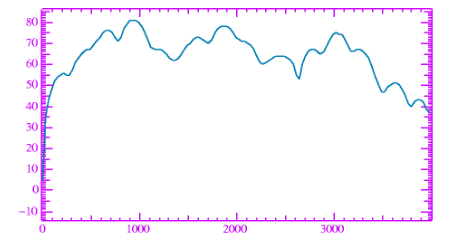
\includegraphics[width=0.6\linewidth]{./graphics/formants.png}
\caption{Representaci\'on del espectro en el cual pueden identificarse los picos espectrales o formantes 
\cite{Jurafsky}.}
\label{figure:formants}
\end{figure}

Los picos espectrales del espectro del sonido se conocen como formantes \cite{Fant1960acoustic}. Distintos fonemas poseen 
formantes a frecuencias determinadas, raz\'on por la cual el an\'alisis espectral tiene un rol determinante en la 
determinaci\'on de la identidad de vocales y otros \mbox{fonemas \cite{LadefogedCourse2006}}.

Un espectrograma como el de la figura~\ref{figure:spectrogram}, por su parte, es una matriz de celdas indexadas por
frecuencia en el eje vertical y por tiempo en el eje 
horizontal, donde el nivel de sombreado de una celda indica la amplitud de la componente a una frecuencia y un tiempo 
dado. Aunque rara vez sean utilizados los espectrogramas para caracterizar directamente la se\~nal,
por resultar poco conveniente en t\'erminos del tama\~no de la representaci\'on,
la gran mayor{\'\i}a de las caracter{\'\i}sticas espectrales utilizadas para el reconocimiento del 
habla est\'an basadas en el \mbox{espectrograma \cite{Ellis08anintroduction}}.

\begin{figure}[H]
\centering
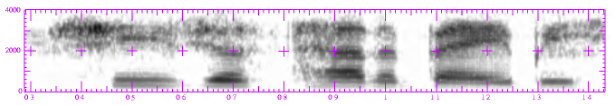
\includegraphics[width=0.9\linewidth]{./graphics/spectrogram.png}
\caption{Representaci\'on gr\'afica de un espectrograma, puede verse como una colecci\'on de espectros como la 
    figura~\ref{figure:formants} ubicados uno despu\'es otro \cite{Jurafsky}.}
\label{figure:spectrogram}
\end{figure}

\subsection{Proceso de Extracci\'on de Caracter{\'\i}sticas}
El proceso puede resumirse en los siguientes pasos \cite{Jurafsky}:

\begin{enumerate}
\item Muestreo: consiste en medir la amplitud de la se\~nal en un momento dado; la frecuencia de muestreo es el 
n\'umero de muestras que se toma por segundo. 

De acuerdo a la f\'ormula de Nyquist, es necesario que la frecuencia de muestreo sea al menos el doble de la frecuencia 
correspondiente a la onda que se desea medir. Por ejemplo, para las conversaciones telef\'onicas, cuyas frecuencias no 
superan los 4000 Hz, una tasa de muestreo de 8000 Hz resulta suficiente.

\item Cuantificaci\'on: consiste en representar el n\'umero real correspondiente a la amplitud 
como un n\'umero entero, normalmente de 8 bits (con valores de -128 a 127) o 16 bits (con valores de -32768 a 32767) para cada muestra. 
Con este paso finaliza la transformaci\'on de anal\'ogico a digital de la se\~nal de voz.

\item Conversi\'on: una vez digitalizada, la se\~nal se convierte a un conjunto de caracter{\'\i}sticas espectrales. Los detalles de este 
paso dependen en gran medida del conjunto de caracter{\'\i}sticas que se selecciona para representar a la se\~nal.

\end{enumerate}

\subsection{Caracter{\'\i}sticas}
Un buen conjunto de caracter{\'\i}sticas espectrales re\'une las siguientes cualidades \cite{KesarkarFeature2003}:
\begin{itemize}
\item Las caracter{\'\i}sticas son perceptualmente significativas, es decir, an\'alogas a las utilizadas 
por el sistema auditivo humano.
\item Las caracter{\'\i}sticas son invariantes, es decir, robustas con respecto a las variaciones en el canal 
y el emisor.
\item Las caracter{\'\i}sticas capturan la din\'amica espectral, es decir, los cambios del espectro en el tiempo.
\end{itemize}

Algunos conjuntos de caracter{\'\i}sticas com\'unmente utilizados son:
\begin{itemize}
\item \gls{lpc}: representaci\'on del espectro basada en la idea de que una muestra 
sonora puede ser aproximada mediante la combinaci\'on lineal de muestras \mbox{anteriores \cite{KesarkarFeature2003}}.
\item An\'alisis Cepstral en escala de Mel: es el conjunto de caracter{\'\i}sticas m\'as com\'unmente utilizado. 
Basado en el concepto de ceptro, una representaci\'on que convierte los efectos del filtrado sobre una onda en una 
operaci\'on de adici\'on. Los coeficientes cesptrales se representan en la escala de Mel, una escala de frecuencia no
lineal de frecuencia basada en la percepci\'on de \mbox{tonos \cite{Ellis08anintroduction}}.
\item An\'alisis Predictivo Lineal Perceptual: se basa en las caracter{\'\i}sticas \gls{lpc} y las modifica de manera 
consistente a la percepci\'on por parte del ser humano. Por ejemplo, se tiene en cuenta los problemas de las personas 
para percibir ondas de alta frecuencia y la relaci\'on entre volumen e intensidad como factores para la 
transformaci\'on de las \mbox{caracter{\'\i}sticas \cite{Jurafsky}}. 
\end{itemize}

La evaluaci\'on y comparaci\'on de estos conjuntos de caracter{\'\i}sticas espectrales para el problema
del reconocimiento del habla es objeto de estudio de numerosos trabajos de
\mbox{investigaci\'on \cite{DorraComparative2006, SarosiComparison2011, ElminirEvaluation2012}}.


\subsection{Resumen}

\begin{figure}[H] 
\centering
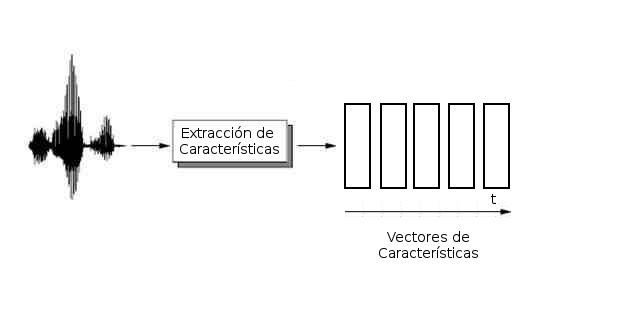
\includegraphics[width=0.8\textwidth]{./graphics/extraccion.png}
\caption{Fase de extracci\'on de caracter{\'\i}sticas. Gr\'afico basado en \cite{VerenichASR}.}
\label{figure:hmm}
\end{figure}

La fase de extracci\'on de caracter{\'\i}sticas inicia con la recepci\'on de una onda sonora,
correspondiente a la voz.
La misma puede caracterizarse mediante los formantes que se observan en un espectrograma.

Durante esta fase se sigue un proceso de an\'alisis de se\~nal: muestreo, cuantificaci\'on y conversi\'on.
Los detalles de este proceso dependen del conjunto de caracter{\'\i}sticas espectrales seleccionado 
para representar la se\~nal.

Al t\'ermino de la fase de extracci\'on de caracter{\'\i}sticas se obtiene un conjunto de vectores 
de caracter{\'\i}sticas espectrales, cada uno de los cuales describe cuantitativamente una trama de
la onda sonora original. Estos vectores representan la entrada de la fase siguiente del proceso del reconocimiento del habla.